\documentclass[11pt,french]{article}
\usepackage{graphicx}
\usepackage{array}
\usepackage[T1]{fontenc}
\usepackage[utf8]{inputenc}
\usepackage{lmodern}
\usepackage[left=2.2cm,right=2.2cm, bottom=2.5cm, top=2.5cm, headheight=2.0cm,footskip=1.5cm,headsep=1cm, heightrounded=true,a4paper]{geometry}
\usepackage{babel}
\usepackage{fancyhdr}
\usepackage{amsmath}
\usepackage{amssymb}
\usepackage{latexsym} 
\usepackage{caption}
\usepackage{siunitx}
\usepackage{tikz}
\usepackage{algorithm}
\usepackage{algpseudocode}
\usepackage{hyperref}
\usepackage{tikz}
\captionsetup[figure]{font=small}
\setlength{\belowcaptionskip}{-10pt}
\captionsetup{belowskip=0.0pt}
\captionsetup{position=below}
\hypersetup{colorlinks=true,citecolor=blue,	urlcolor=black,linkcolor=black}
\usepackage{graphicx}
\graphicspath{{images/}} 
\usepackage{placeins}

\title{TP\_CR}
\author{Adrien Taberner}
\date{ \today}
\begin{document}
	
	\begin{center}
		\vspace*{15pt}
		\huge
		\textbf{Rapport méthode de Lanczos}\\
		\vspace{15pt}
		\LARGE
		Algorithme de Lanczos pour des matrices Hermitienne\\
		\vspace{10pt}	
		\large
		 Mounir Cherif \& Adrien Taberner  \\ 
		 \today  \\
		\vspace{5pt}	
	\end{center} 
	
	\vspace{30pt}	
	\tableofcontents
	
	\newpage
	
	\renewcommand{\headrulewidth}{0.4pt}
	\renewcommand{\footrulewidth }{0.4pt}
	\fancyfoot[C]{}
	\fancyfoot[R]{\thepage}
	\fancyfoot[L]{ Mounir Cherif \& Adrien Taberner}
	\fancyhead[L]{MPNA}
	
	\section{Introduction}
		\pagestyle{fancy}
	\par En algèbre linéaire l'algorithme de Lanczos est une méthode itérative. Elle se présente comme une variante de l'algorithme d'Arnoldi, spécifiquement adaptée aux matrices symétriques et hermitiennes. Une caractéristique de cet algorithme réside dans la transformation de la matrice initiale, qui passe d'une forme Hessenberg supérieure à une forme tridiagonale. \\

	\par L'amélioration apportée par l'algorithme de Lanczos par rapport à ses prédécesseurs se manifeste dans la manière dont chaque vecteur $v$ est construit. Dans cette approche, chaque $v$ est restreint à être orthogonal à tous les vecteurs générés précédemment. Pendant la construction de ces vecteurs, les constantes de normalisation sont regroupées dans une matrice tridiagonale. Les valeurs propres les plus significatives de cette matrice convergent rapidement vers celles de la matrice d'origine. \\

	\par Cette méthodologie offre un avantage majeur, limitant l'opération de grande envergure à la multiplication par la matrice $A$. Ainsi, l'algorithme de Lanczos simplifie le processus, concentrant l'intérêt sur cette opération cruciale. \\
	
	\section{Problématique}
	\par L'algorithme de Lanczos s'inscrit dans le contexte de la recherche des valeurs propres et des vecteurs propres dominantes d'une matrice symétrique ou hermitienne.
 
    Plusieurs défis doivent être relevés pour utiliser efficacement l'algorithme de Lanczos :
    \begin{itemize}
    \item \textbf{Choix de la taille de la sous-matrice :} La taille de la sous-matrice utilisée dans l'algorithme de Lanczos est un compromis entre la précision et le coût computationnel.

     \item \textbf{Perte d'orthogonalité :} L'algorithme de Lanczos peut souffrir de la perte d'orthogonalité des vecteurs générés au fil des itérations, ce qui peut affecter la convergence et la précision de l'algorithme. Des techniques telles que la réorthogonalisation complète peuvent être utilisées pour atténuer ce problème.
    
    \end{itemize}
	\section{Approche utilisé}
	
	\subsection{Représentation mémoire d'une matrice symétrique}
	Avec une matrice symétrique à coefficients réels, la moitié des coefficients, en plus de la diagonale, peuvent être présent en mémoire. La figure ci-dessous illustre les éléments qui sont enregistrés en mémoire.
		\begin{figure}[h]
		\centering
		$A _{n, n}=
		\begin{pmatrix}
			a_{1,1} & a_{1,2}& \cdots & \cdots & a_{1,n} \\  
			   & a_{2,2} & \cdots & \cdots & a_{2,n} \\  
			   &   & \ddots &   & \vdots \\  
			   &   &   & \ddots & \vdots \\  
			   &   &   &   & a_{n,n}\\  
		\end{pmatrix}
		$
	\end{figure}
	 \newpage 
	\section{Cas Séquentiel}
	
	\subsection{Description de l'algorithme}
	\begin{algorithm}
		\caption{Algorithme de Lanczos}\label{alg:lanczos}
		\begin{algorithmic}[1]
			\Require {$A$ une matrice de dimension $n$  symétrique }
			\Require {Choisir $v_0$ un vecteur initial et $\beta_0$ un réel}
			\State $v_1 \gets v_0 \times|| v_0||^{-1} $
			\For{ $j = 1, 2, 3, ..., m$}
				\State $w_j \gets Av_j - \boldsymbol{\beta_j }v_{j-1}$
				\State $\boldsymbol{\alpha_j} \gets (w_j,v_j)$
				\State $w_j \gets w_j - \boldsymbol{\alpha_j} v_j$
				\State $\boldsymbol{\beta_{j+1}} \gets || w_j||_2$
				\State $ v_{j+1} \gets w_j /\boldsymbol{\beta_{j+1}} $
			\EndFor
			\State \Return 
		\end{algorithmic}
	\end{algorithm}
	
	\subsection{Évaluation des performances théoriques}
	Une métrique fréquemment utilisée est le débit \emph{(throughput)} des opérations flottantes effectuées. L’acronyme \textbf{\emph{flop}} qui signifie \emph{"Floating Point Operation"} est habituellement utilisé pour mesurer la capacité du système à effectuer une opération arithmétique à virgule flottante. Le nombre d'opérations réalisées par l'algorithme sera ainsi calculé dans la suite du paragraphe.  \\

	\noindent \textbf{Ligne  3}
	cette ligne trois opérations sont réaliser : un produit matrice-vecteur, un produit scalaire et une addition de vecteurs. \\ \\
	$\boldsymbol{ A \times v_j}$\\
	Le nombre d’éléments de la matrice est de $n^2$ mais de $\frac{n^2 + n}{2}$  en mémoire.\\
	Il y a deux opération par éléments :  un produit avec un élément du vecteur  $v_j$ et une somme avec un élément de $w_j$.
	Donc $2n^2$ opérations pour cette instruction. \\ \\
	$\boldsymbol{ - \beta_j \times v_{j - 1}}$\\
	Les opérations réalisées sont un produit scalaire et une addition sur un vecteur de taille $n$.
	Donc il y a $2n$ flop pour cette instruction. \\  \\
	\noindent $\boldsymbol{w_j \gets Av_j - \beta_j  v_{j-1}}$ \\
	Il y a donc $2n^2 + 2n$ opération flottante pour la ligne 3 de l'algorithme.  \\
	
	\noindent \textbf{Ligne  4}\\
	$\boldsymbol {\alpha_j \gets (w_j,v_j)}$
	Cette instruction correspond a un produit de deux éléments puis une réduction sur l'ensemble du vecteur. Il y a donc $2n$ flop pour cette ligne. \\
	
	\noindent\textbf{Ligne  5}\\
	$\boldsymbol {w_j - \boldsymbol{\alpha_j} v_j}$
	La ligne 5 est composé de deux  opération un produit scalaire et une somme de vecteur, ce qui donne $2n$ flop. \\
	
	\noindent\textbf{Ligne  6}\\
	$\boldsymbol {\beta_{j+1} \gets || w_j||_2}$
	Cette instruction correspond a un produit de chaque élément de $w_j$ puis d'une réduction des $n$ éléments. Il y a donc $2n$ flop pour cette ligne.  \\
	
	\noindent\textbf{Ligne  7}\\
	$\boldsymbol {v_{j+1} \gets w_j \beta_{j+1}}$
	La ligne 7 est composé d'un produit scalaire entre l’inverse de $\beta_{j+1}$ et le vecteur $w_j$, ce qui donne $n$ flop pour cette instruction. \\ 
	
	\noindent\textbf{Opération flottante par itération}
	Pour chaque ligne de l'algorithme \ref{alg:lanczos} on a obtenue le nombre d’opérations flottante  $2n^2 + 2n + 2n +2n +2n +n = 2n^2 + 9n$. Ce nombre d’opérations dépend de la dimension de la matrice et est majoré par le terme $n^2$, ce terme provient du produit matrice vecteur de la ligne 3. \\
	
	\noindent \textbf{Opérations flottante total}. Le nombre d’opération pour l'ensemble de l'algorithme de Lanczos dépend du choix de $m$, la taille de la matrice en sortie.\\ 
	Le nombre de flop est donc de : $  m(2n^2 + 9n) \quad flop $
	
	\subsection{Évaluation des performances pratiques}
	Les performances sont mesurées sur un cœur du processeur Intel Xeon Gold 6230.

    Le tableau suivant montre les résultats d'un test pour une matrice d'entrée de taille $n=5000$, dans ce test nous mesurons le temps d'exécution et le Gflops en fonction de la taille de la matrice de sortie $m$.
    \begin{table}[htbp]

    \centering
    \begin{tabular}{ |p{3cm}|p{3cm}|p{3cm}|  }
    \hline
    m & Time & Gflops \\
    \hline
    5   &  0.1228   &  9.0377\\
    10   &  0.2269  &   8.8052\\
    15   &  0.3704  &   7.0268\\
    20   &  0.4513  &   6.4177\\
    25   &  0.4929  &   4.1462\\
    30   &  0.5495  &   2.7133\\
    35  &   0.6277  &   2.8880\\
    40   &  0.6555  &   2.0950\\
    45    & 0.7281  &   1.9052\\
    50   & 0.7839  &   1.8901\\
    \hline
    \end{tabular}
    \captionof{table}{Variation de temps d'exécution et de Gflops en fonction de la taille de la matrice de sortie $m$}
    \end{table}

    Les figures suivantes représentent les résultats du tableau précédent :
    \begin{figure}[h]
    \centering
    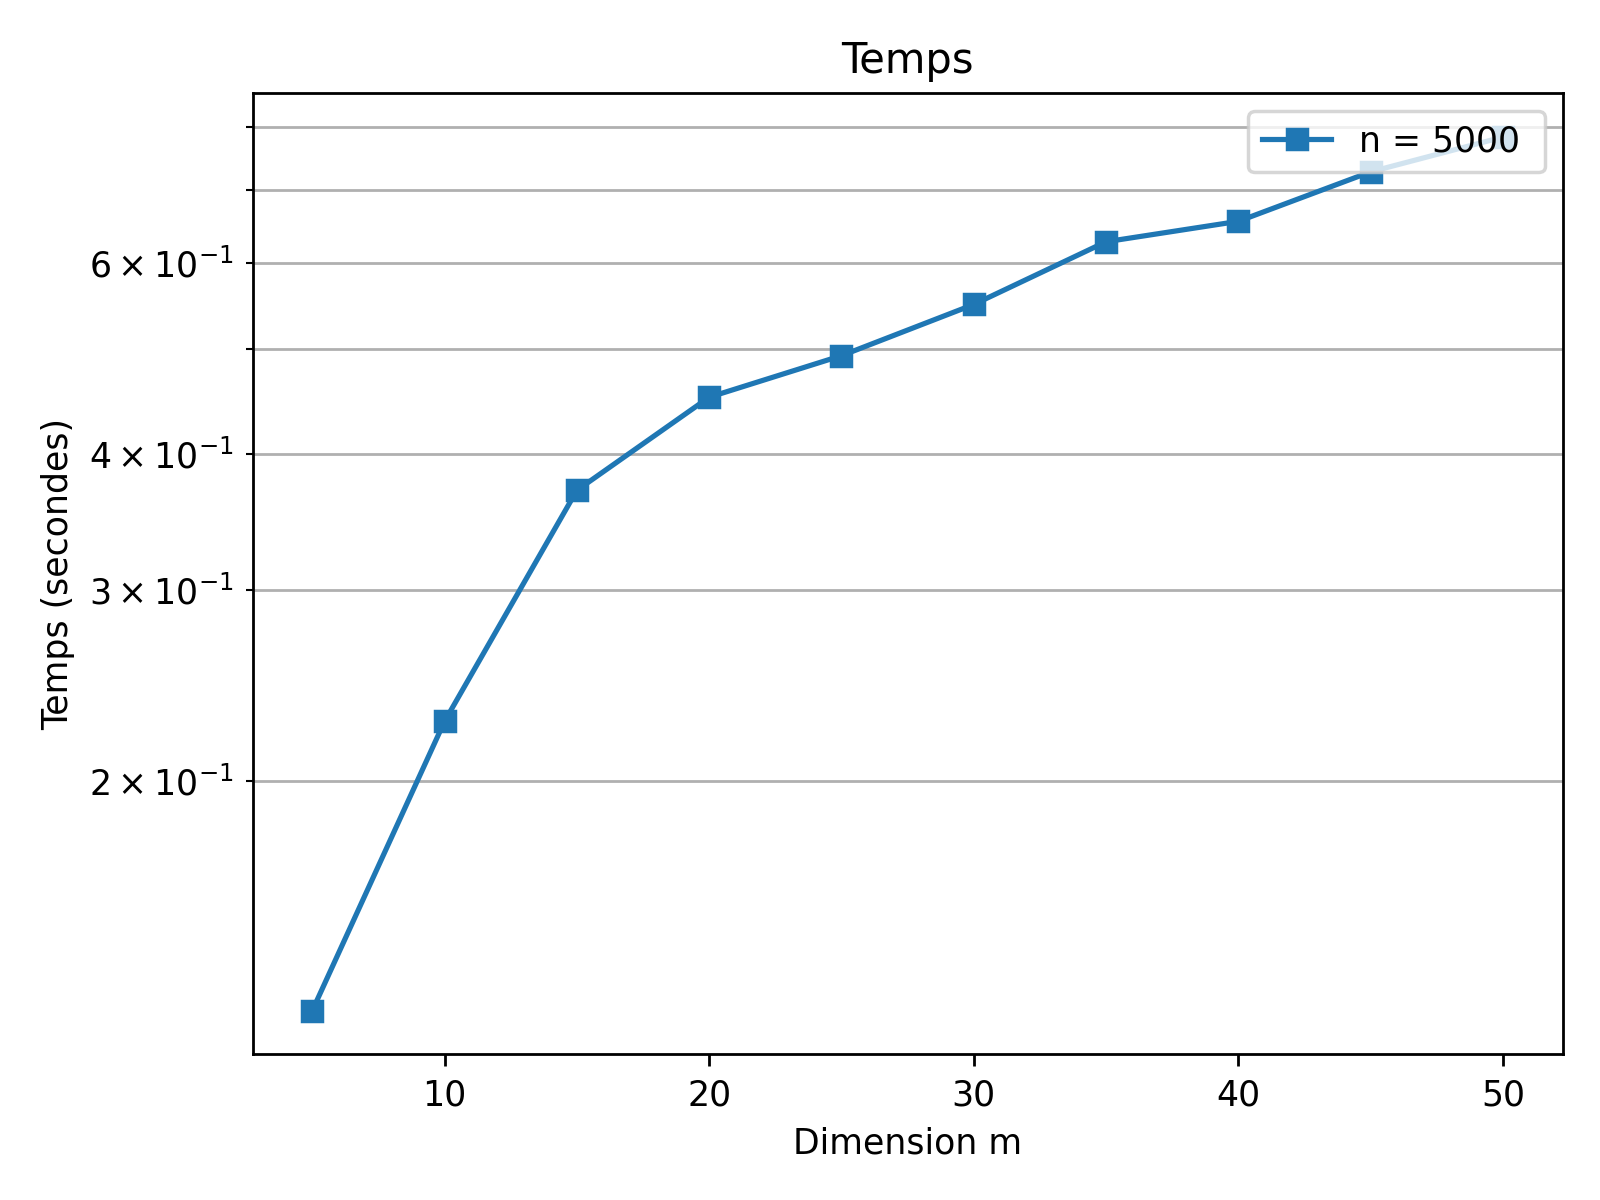
\includegraphics[width=0.7\textwidth]{Images/m_Time.png}
    \caption{Temps d'exécution en fonction de $m$}
    \label{fig:mesh1}
    \end{figure}
    \FloatBarrier
    
    La figure montre le temps de calcul en fonction de la taille de la matrice de sortie $m$ pour une matrice hermitienne de taille n = 5000. Le graphique est divisé en deux zones, une zone où le temps de calcul augmente rapidement et une zone où le temps de calcul augmente lentement (à partir de $m=20$).
    En regardant le graphique, on peut voir que le temps de calcul est relativement faible pour un nombre d'itérations de $<20$. Pour $m=50$, le temps de calcul est déjà plus important. 
    \begin{figure}[h]
    \centering
    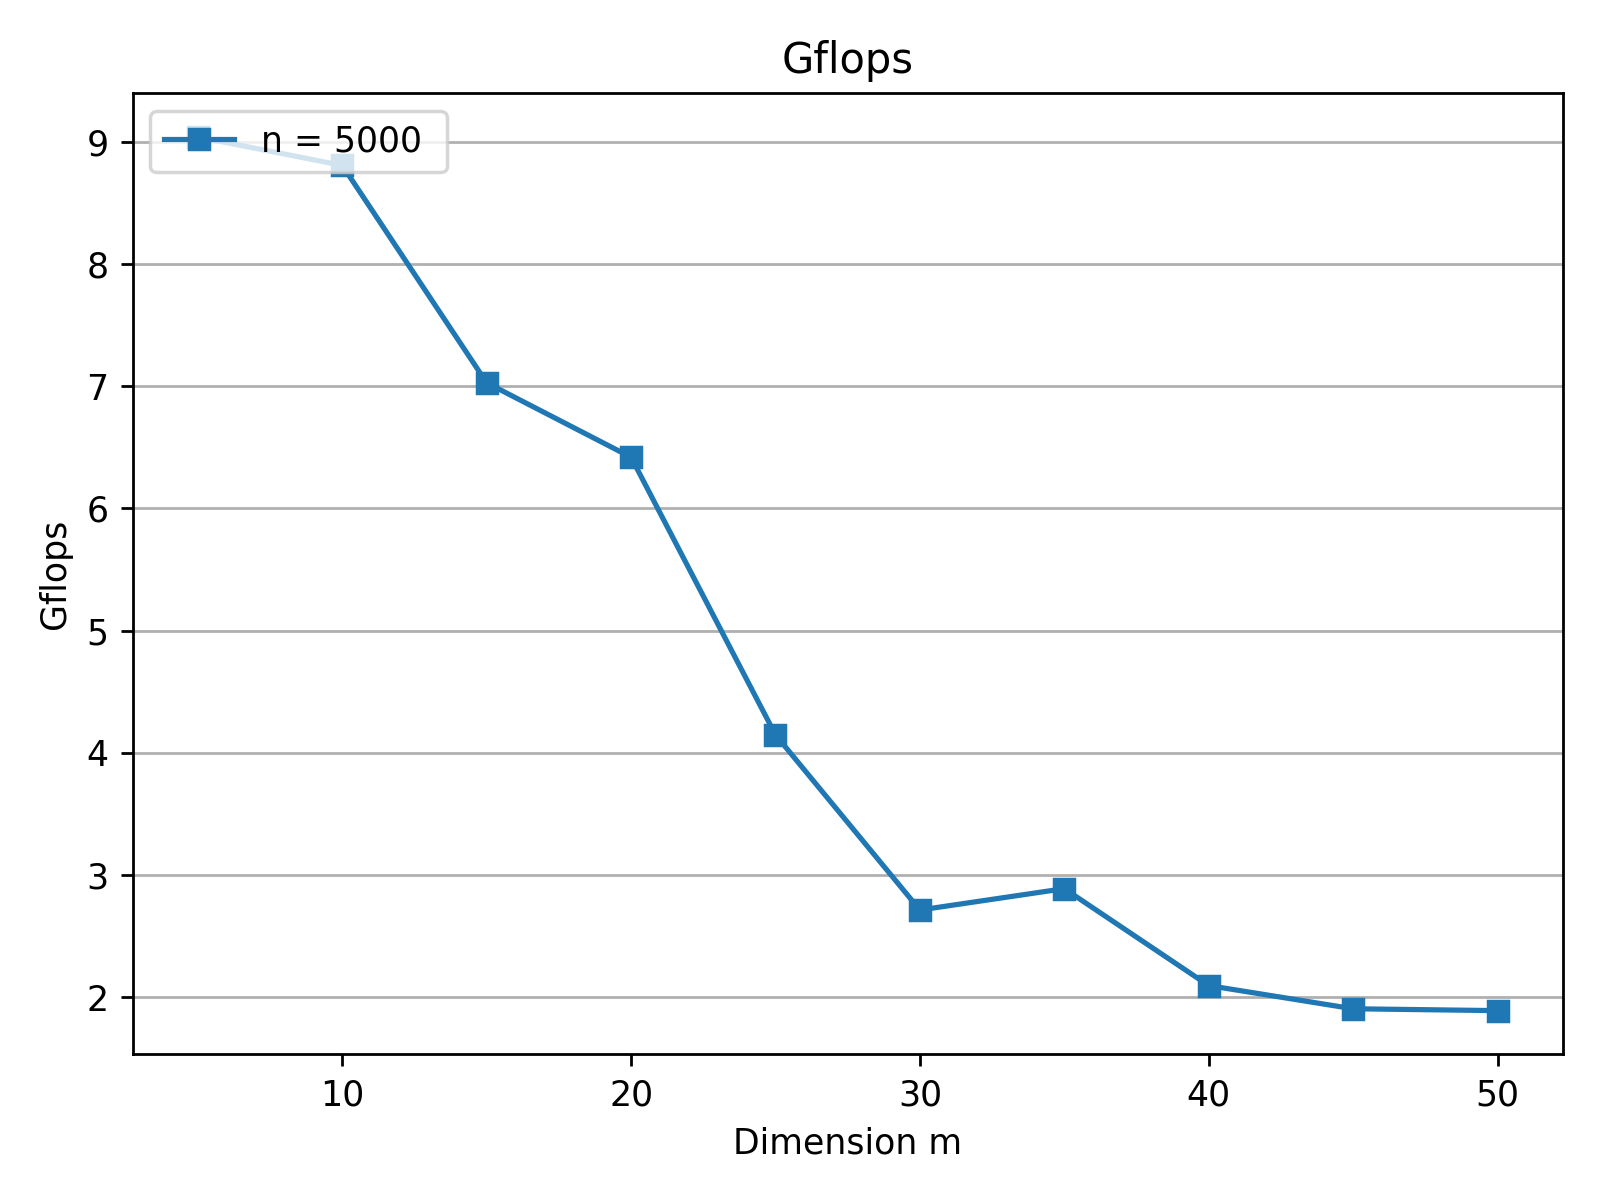
\includegraphics[width=0.7\textwidth]{Images/m_Gflops.png}
    \caption{Gflops en fonction de $m$}
    \label{fig:mesh1}
    \end{figure}
    \FloatBarrier
    
    Le graphe montre le nombre de flops (floating point operations) en fonction de la taille de la matrice de sortie $m$ pour une matrice hermitienne de taille n = 5000. Le graphique est divisé en deux zones, une zone où le nombre de flops diminue rapidement et une zone où le nombre de flops diminue lentement ($m>30)$.
    \FloatBarrier
    
	\newpage

	\section{Cas parallèle}
	
	\subsection{Description}
    C'est une extension de l'algorithme de base conçue pour exploiter les capacités de traitement parallèle des systèmes informatiques modernes. Le parallélisme permet d'accélérer la convergence de l'algorithme et donc d'augmenter son efficacité pour la résolution de grands problèmes.

    Voici une description générale du cas parallèle de l'algorithme de Lanczos :
    \begin{itemize}

    \item \textbf{Parallélisation des calculs :} Dans l'algorithme de base de Lanczos, les calculs des vecteurs propres sont généralement effectués de manière séquentielle. Dans le cas parallèle, ces calculs sont répartis entre plusieurs processeurs ou cœurs de calcul, ce qui permet d'effectuer plusieurs calculs simultanément.
    \item \textbf{Décomposition de la matrice :} Pour exploiter le parallélisme, la matrice d'origine est souvent décomposée en sous-matrices plus petites qui peuvent être traitées de manière indépendante par différents processeurs. Cette décomposition peut être réalisée de différentes manières en fonction de la structure de la matrice et des ressources disponibles.
    \item \textbf{Communication entre les processus :} Comme les différents processus travaillent sur des parties distinctes de la matrice, il est souvent nécessaire d'échanger des informations entre eux à certaines étapes de l'algorithme. Une communication efficace entre les processus est essentielle pour garantir la cohérence des résultats et éviter les goulots d'étranglement.
    \item \textbf{Gestion des ressources :} L'utilisation efficace des ressources parallèles est un aspect crucial du cas parallèle de l'algorithme de Lanczos. Cela implique une répartition équilibrée des tâches entre les différents processeurs.
	\end{itemize}

    \subsection{Architecture parallèle visée}
    Dans cette section, nous présentons l'architecture parallèle visée pour l'implémentation de l'algorithme de Lanczos. L'architecture parallèle fait référence à la configuration matérielle et logicielle sur laquelle l'algorithme sera exécuté. Pour notre étude, nous avons choisi d'utiliser OpenMP, une API de programmation parallèle pour les architectures à mémoire partagée.
    
    Elle permet d'exploiter facilement le parallélisme au niveau des boucles, des sections de code et des tâches, en utilisant des directives de compilation et des bibliothèques spécifiques. L'utilisation d'OpenMP offre une approche flexible et portable pour le développement de codes parallèles.
    
    Pour implémenter l'algorithme de Lanczos en parallèle avec OpenMP, nous prévoyons d'exploiter le parallélisme au niveau des boucles internes de l'algorithme. Les étapes de calcul intensif, telles que la multiplication de matrices et le calcul des produits scalaire, seront parallélisées pour exploiter efficacement les ressources de calcul disponibles
    
	\subsection{Évaluation des performances théoriques}
	La complexité de l'algorithme parallèle de Lanczos dépend principalement de la taille de la matrice d'entrée, notée $n$, et de la taille de la matrice en sortie, notée $m$.

    Dans un contexte parallèle, il est essentiel de souligner que des communications et des synchronisations entre les différents threads sont inévitables:
    \begin{itemize}
    \item \textbf{pragma omp parallel for}:  Lors de l'exécution de l'instruction #pragma omp parallel for, le nombre total d'itérations de la boucle est divisé entre les threads disponibles. Cela nécessite une communication entre les threads pour déterminer quelles itérations sont assignées à chaque thread.
    
    \item \textbf{pragma omp parallel for reduction}:  À la fin de la boucle, une opération de réduction est effectuée sur les résultats partiels pour obtenir le résultat final. Cette opération de réduction implique une communication entre les threads pour agréger les résultats partiels.
	\end{itemize}
	\subsection{Évaluation des performances pratiques}
    Les performances sont mesurées sur un cœur du processeur Intel Xeon Gold 6230.

    Le tableau suivant montre les résultats d'un test pour une matrice d'entrée de taille $n=20000$ et une matrice de sortie de taille $m=30$, dans ce test nous mesurons le temps d'exécution et le Gflops en fonction de nombre de threads.
    \begin{table}[htbp]

    \centering
    \begin{tabular}{ |p{3cm}|p{3cm}|p{3cm}|  }
    \hline
    Threads & Time & Gflops \\
    \hline
     1  &  37.6359  &   2.5510\\
     2  &  28.8630  &   3.3264\\
     4  &  16.8191  &   5.7085\\
     8  &   9.2668  &  10.3607\\
    12  &   6.4359  &  14.9179\\
    16  &   4.9434  &  19.4218\\
    24  &   3.4276  &  28.0113\\
    32  &   2.7579  &  34.8130\\
    40  &   2.4658  &  38.9374\\
    \hline
    \end{tabular}
    \captionof{table}{Variation de temps d'exécution et de Gflops en fonction de nombre de Threads}
    \end{table}

    Les figures suivantes représentent les résultats du tableau précédent :
    \begin{figure}[h]
    \centering
    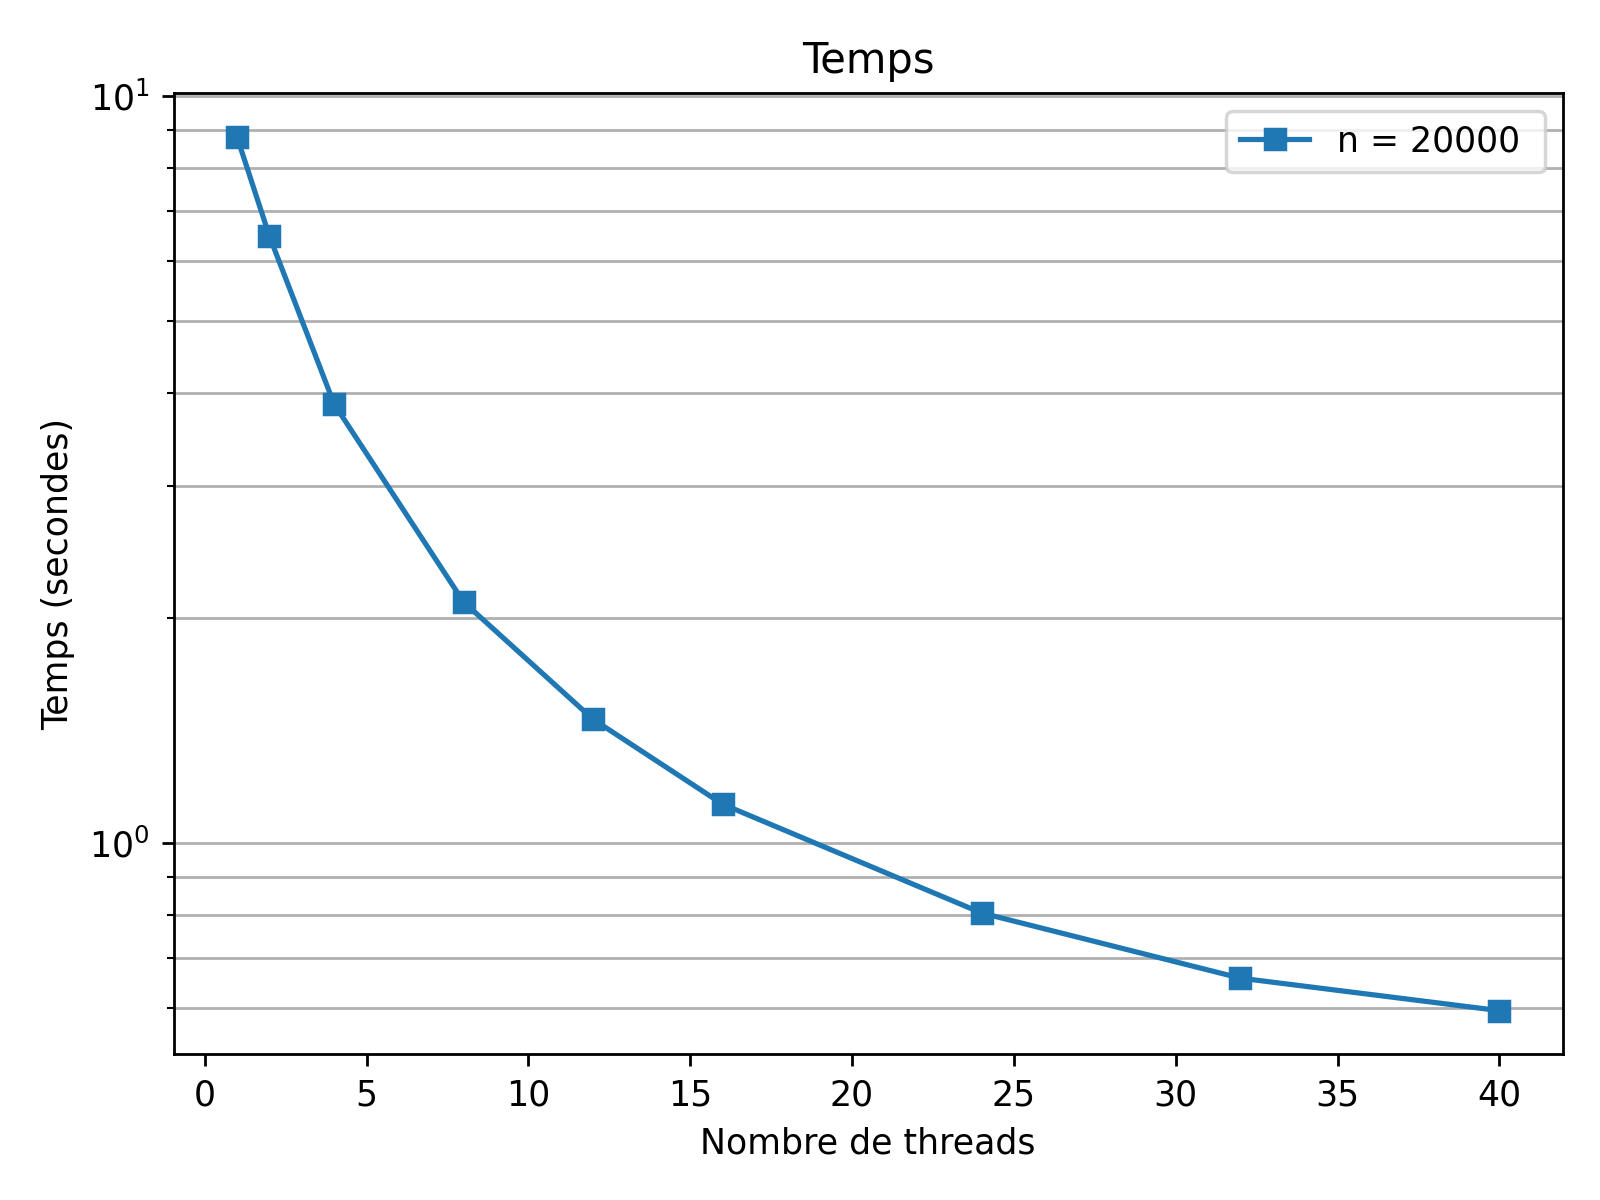
\includegraphics[width=0.7\textwidth]{Images/OMP_Time.png}
    \caption{Temps d'exécution en fonction de nombre de threads}
    \label{fig:mesh1}
    \end{figure}
    \FloatBarrier
    
    La figure montre le temps de calcul en fonction du nombre de threads pour $n = 20000 et m = 30$. Le graphe montre que le temps de calcul diminue rapidement avec l'augmentation du nombre de threads.
    
    Cette amélioration est due au fait que l'algorithme de Lanczos est un algorithme naturellement parallélisable. Les étapes de l'algorithme peuvent être exécutées indépendamment sur différents threads.
    \begin{figure}[h]
    \centering
    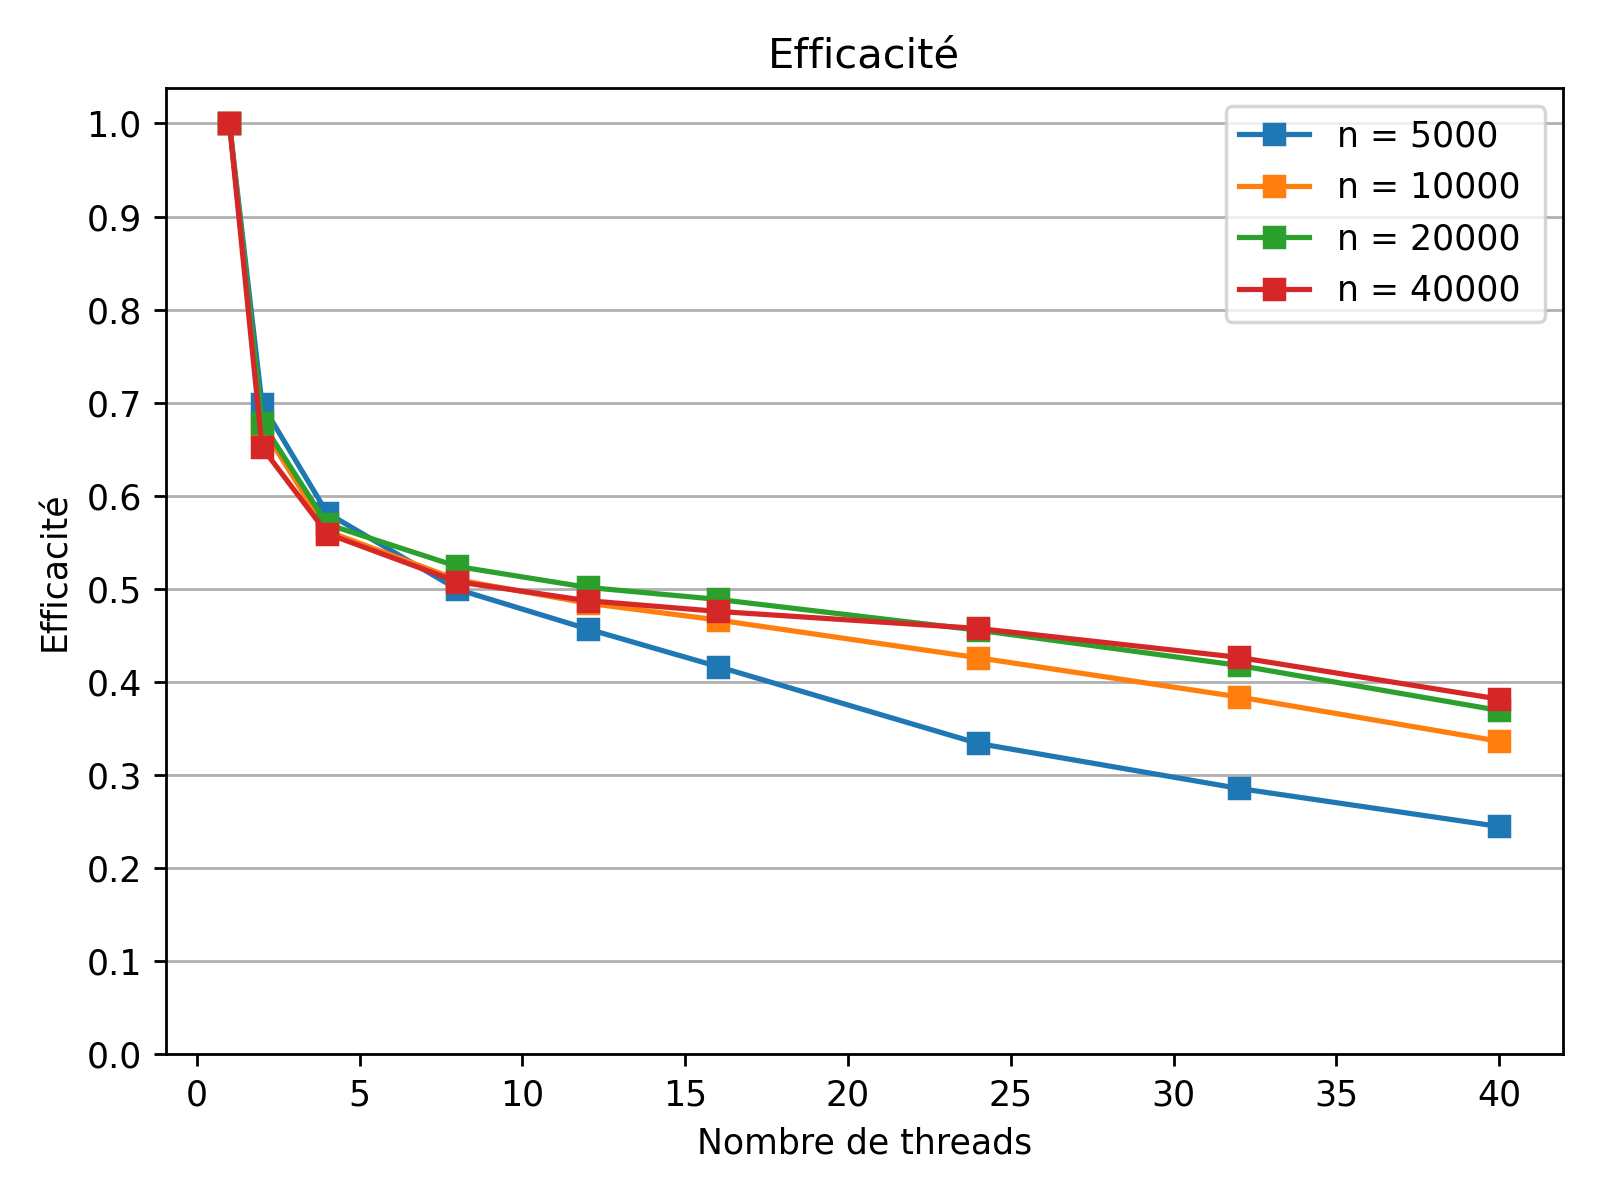
\includegraphics[width=0.7\textwidth]{Images/OMP_Efficiency.png}
    \caption{Efficacité en fonction de nombre de threads}
    \label{fig:mesh1}
    \end{figure}
    \FloatBarrier
    
    Le graphe montre que l'efficacité diminue avec l'augmentation du nombre de threads. Cette diminution d'efficacité est due à plusieurs facteurs, notamment :
    \begin{itemize}
        \item La communication entre les threads.
        \item La contention des ressources.
    \end{itemize}
    
    Il est important de prendre en compte ces facteurs lors de l'optimisation de l'algorithme de Lanczos pour la parallélisation.
    \begin{figure}[h]
    \centering
    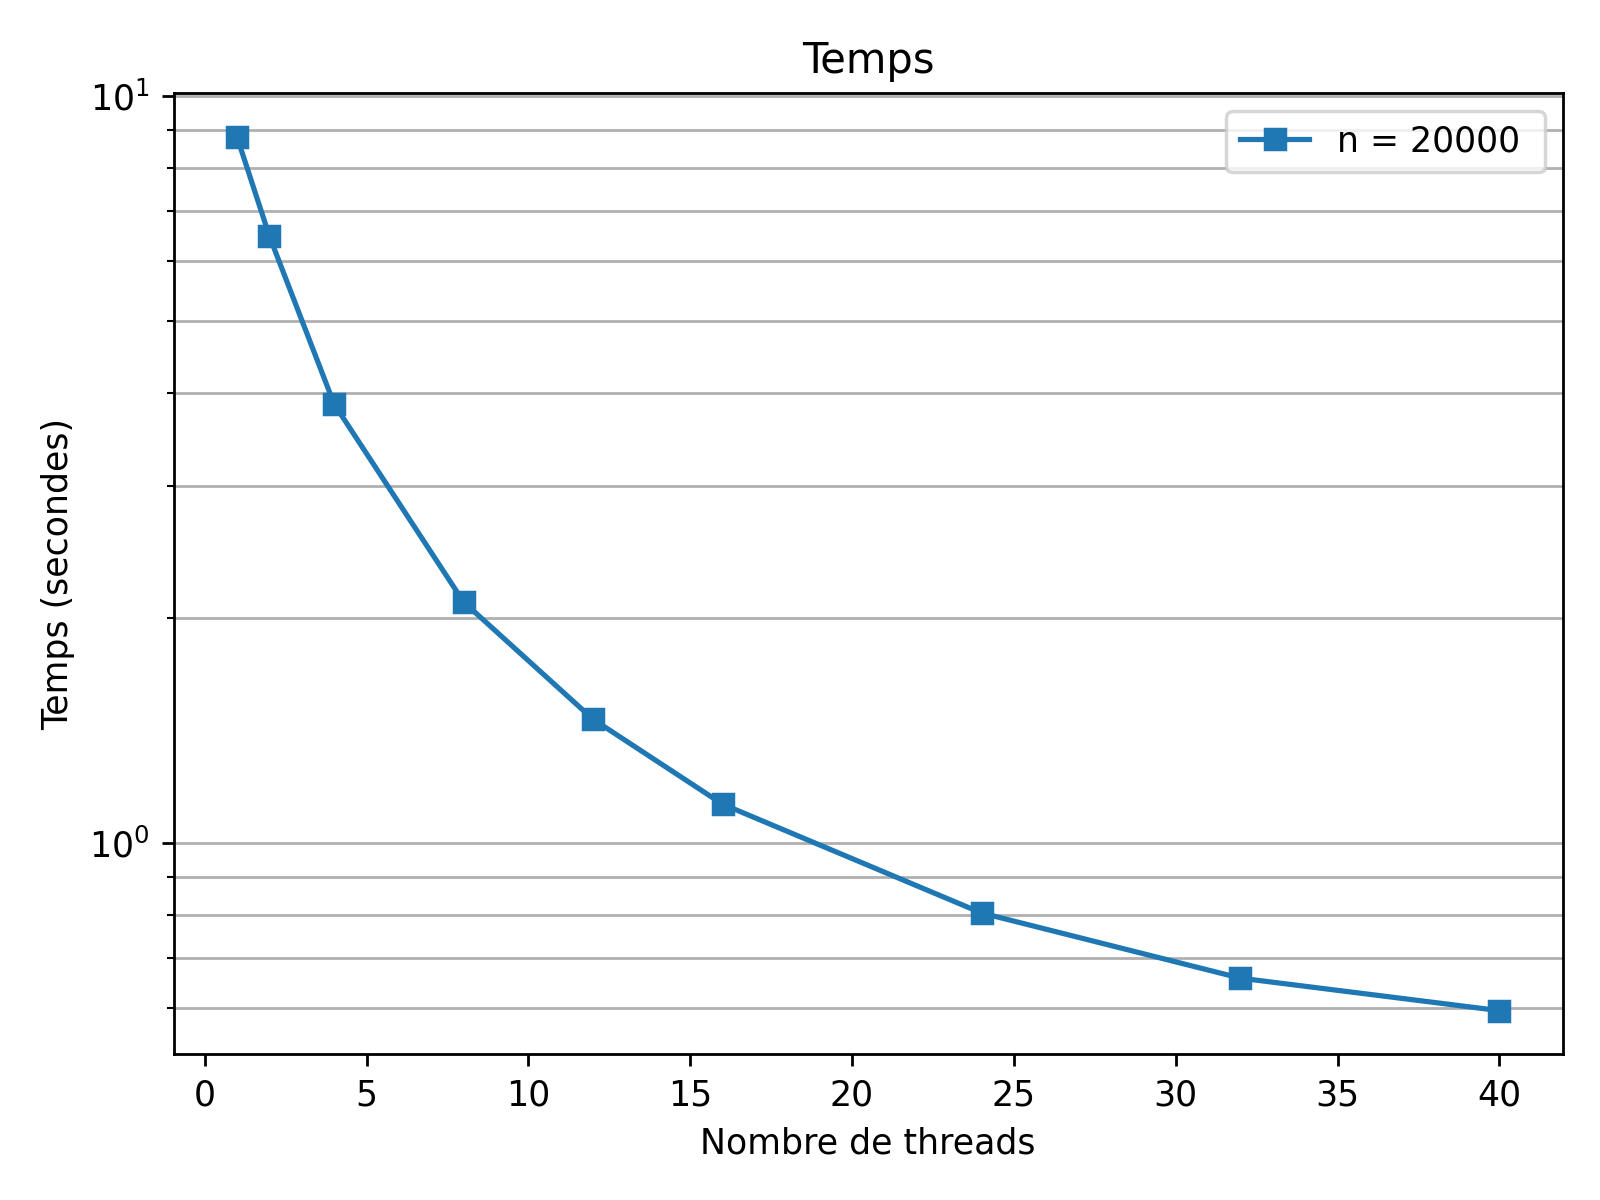
\includegraphics[width=0.7\textwidth]{Images/OMP_Time.png}
    \caption{Gflops en fonction de nombre de threads}
    \label{fig:mesh1}
    \end{figure}
    \FloatBarrier
    
    \begin{figure}[h]
    \centering
    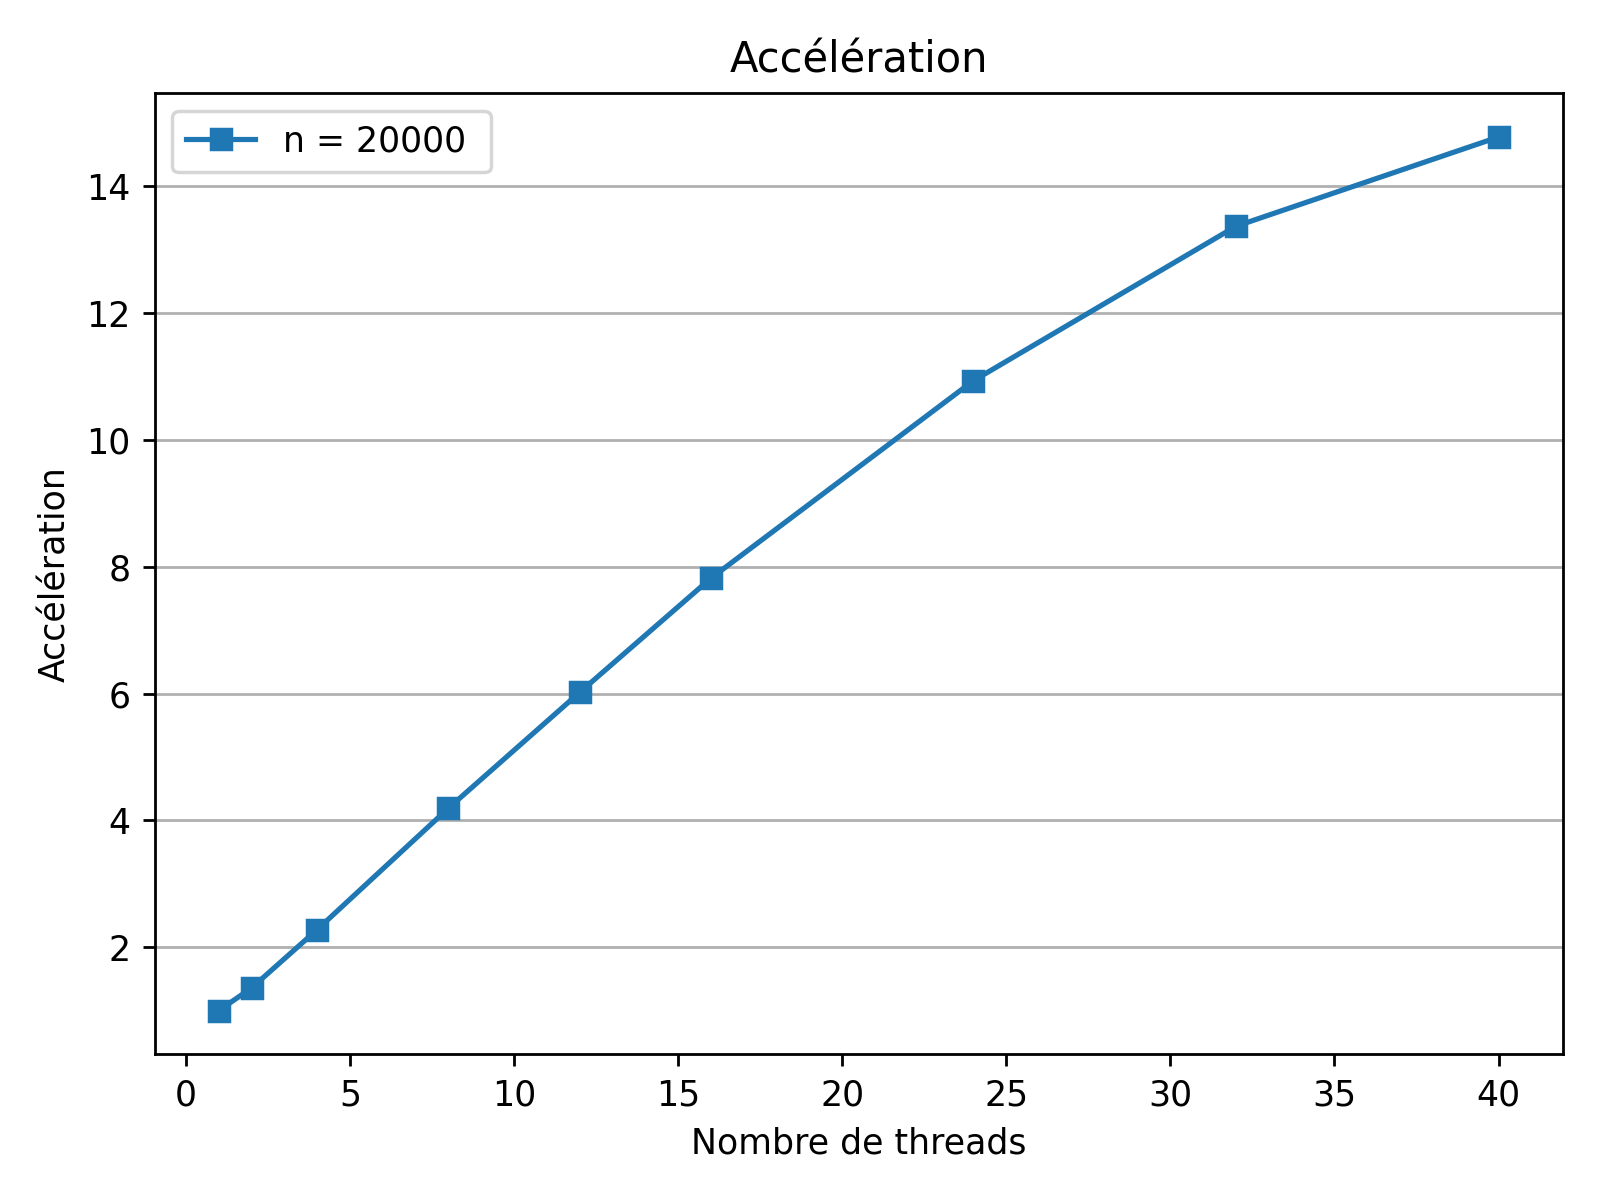
\includegraphics[width=0.7\textwidth]{Images/OMP_SpeedUp.png}
    \caption{Accélération en fonction de nombre de threads}
    \label{fig:mesh1}
    \end{figure}
    \FloatBarrier
    
    La figure montre que l'accélération augmente avec le nombre de threads. Cela est dû au fait que l'algorithme de Lanczos est un algorithme parallélisable. Cela signifie qu'il peut être exécuté sur plusieurs threads simultanément. Lorsque le nombre de threads augmente, l'algorithme peut traiter plus de données en même temps, ce qui entraîne une augmentation de la performance.
    \FloatBarrier
	\newpage
	\section{Conclusion générale}
	L'algorithme de Lanczos est une méthode numérique utilisée pour calculer de manière efficace les valeurs propres d'une matrice symétrique ou hermitienne. Il est relativement simple à implémenter, et il est souvent utilisé en calcul scientifique et en analyse des données pour résoudre des problèmes impliquant de grandes matrices.

    La perte d'orthogonalité est un problème commun dans l'algorithme de Lanczos, ainsi que dans d'autres méthodes itératives pour résoudre des systèmes linéaires ou calculer des valeurs propres. Cette perte d’orthogonalité est un signe de perte d’indépendance linéaire des vecteurs propres. Une fois que cette indépendance est perdue, il commence à apparaître plusieurs copies de la même valeur propre (et du vecteur propre correspondant), qui a convergé.

    La stratégie de réorthogonalisation complète est une technique utilisée pour atténuer la perte d'orthogonalité dans les algorithmes itératifs, tels que l'algorithme de Lanczos. L'idée est de réorthogonaliser chaque $v_{j+1}$ par rapport à tous les $v_i$ précédents.

    L'algorithme de Lanczos est un algorithme parallélisable. Cela signifie qu'il peut être exécuté sur plusieurs threads simultanément. L'utilisation de plus de threads peut entraîner une augmentation significative de la performance.
     
     L'algorithme de Lanczos converge généralement rapidement vers les valeurs propres les plus importantes de la matrice, ce qui en fait une méthode efficace pour résoudre des problèmes de grande taille.

\end{document}
